%\documentclass{standalone}
%\usepackage{tikz}
%\usepackage{amsmath}
%\usepackage{amssymb}
%\begin{document}
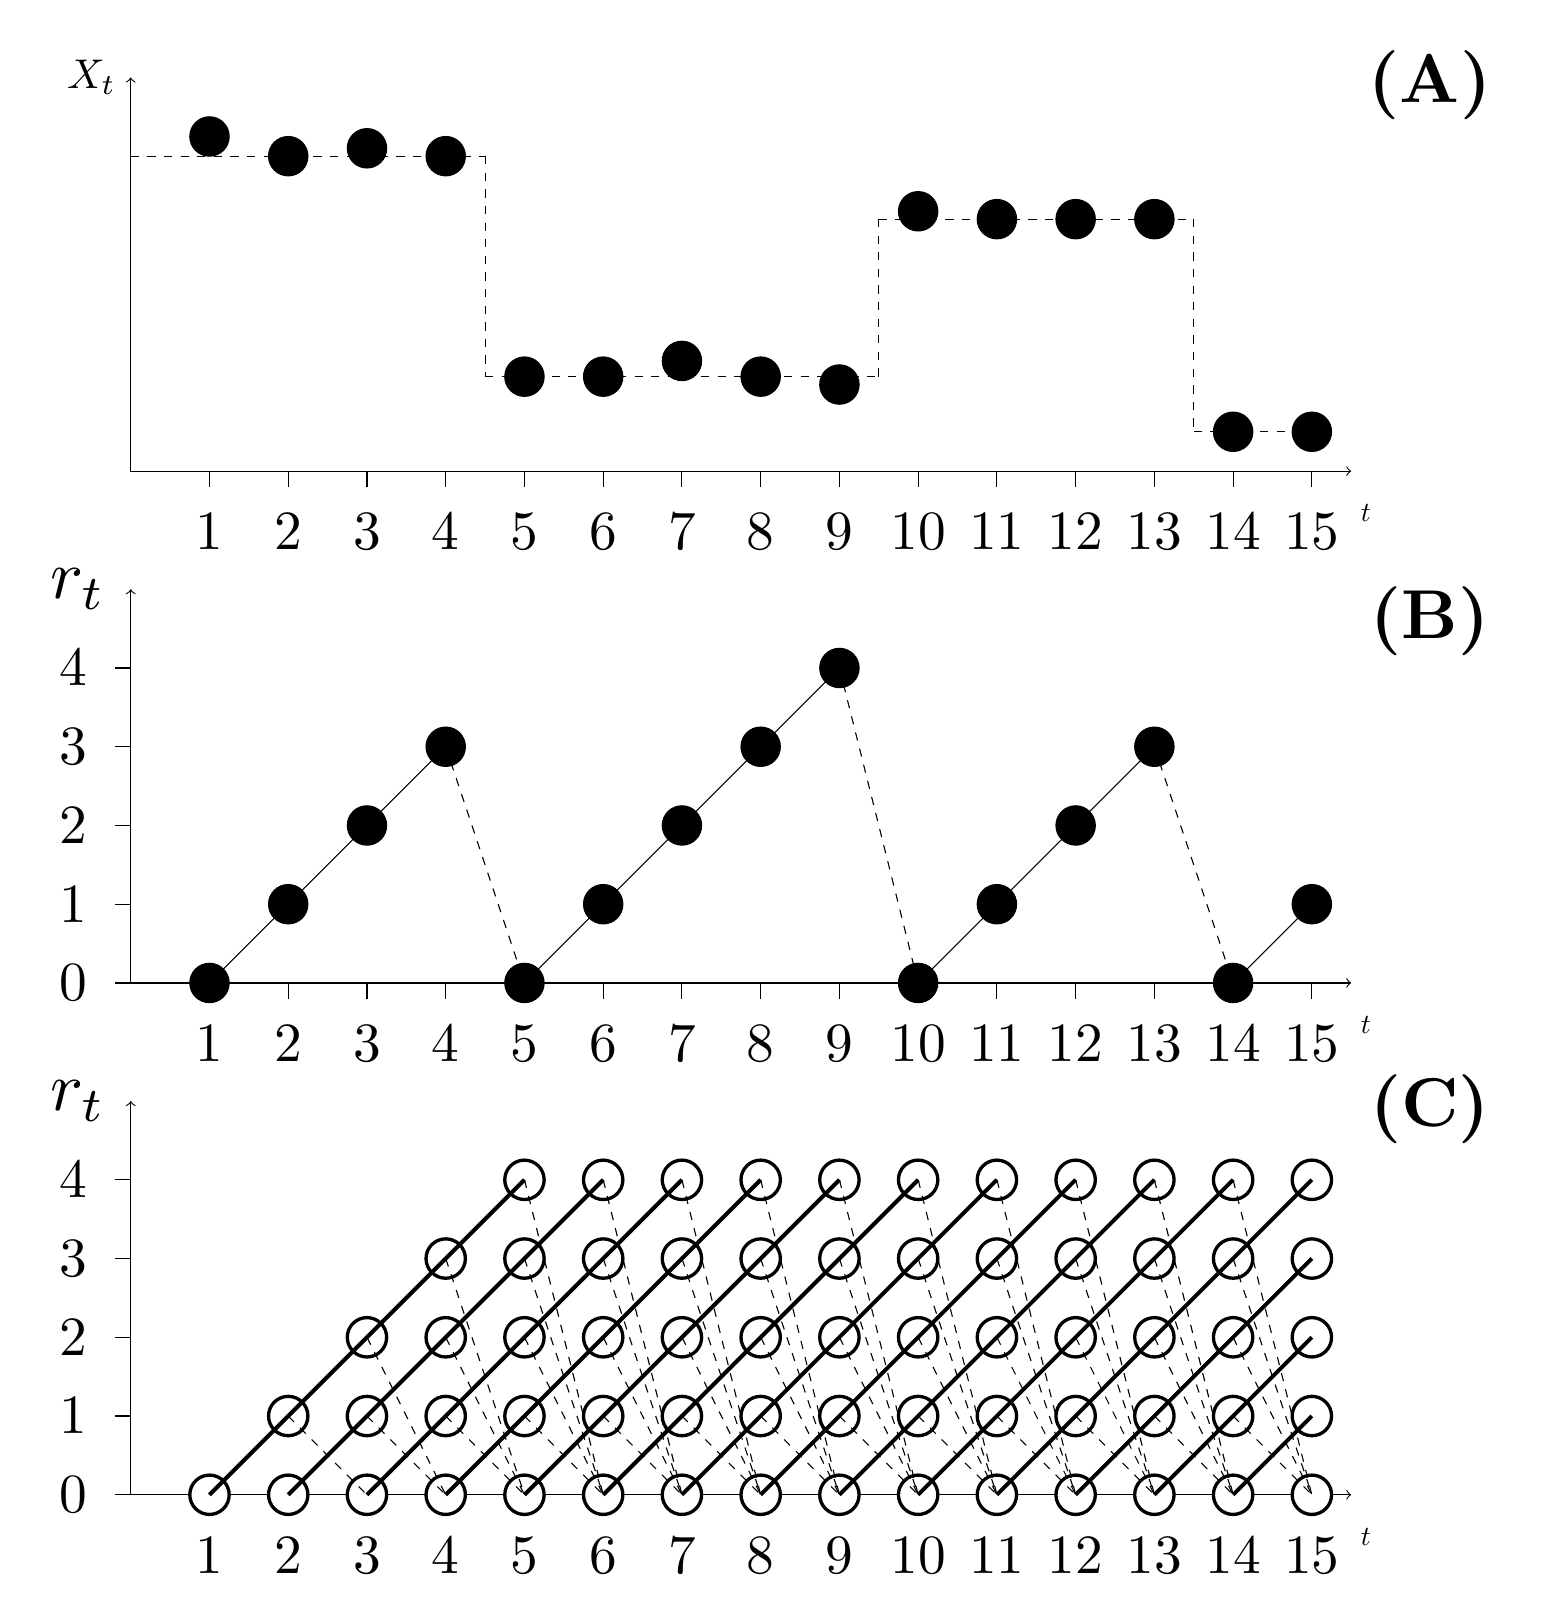
\begin{tikzpicture}[scale=1.0, xscale=1]
\def\ticksz{0.2};
\def\rad{0.25};
\def\shft{6.5};
% LETTERS

\def\lpos{16.5};
\node[scale=2.5](text) at (\lpos, 3*\shft-1.6) {\textbf{(A)}}; 
\node[scale=2.5](text) at (\lpos, 2*\shft-1.9) {\textbf{(B)}}; 
\node[scale=2.5](text) at (\lpos, \shft-1.6) {\textbf{(C)}}; 


%%%%%%%%%%%%%%%%%%%% III PLOT:
\draw [<->] (0, 5+2*\shft) node[left,scale=1.5] {$\pmb{X_t}$} -- (0,0+2*\shft) -- (15.5, 0+2*\shft) node [below right] at (15.5,-0.3+2*\shft) {$t$};
\foreach \x in {1,...,15}{
    \draw (\x, 2*\shft) -- (\x, 2*\shft-\ticksz); 
    \node[below,scale=2] at (\x, 2*\shft-0.3) {\x};}
    
% plot signal 1st part
\def\a{4};
\draw[fill=black] (1, 2*\shft + \a + 0.25) circle (\rad); 
\draw[fill=black] (2, 2*\shft + \a + 0.00) circle (\rad);
\draw[fill=black] (3, 2*\shft + \a + 0.10) circle (\rad);
\draw[fill=black] (4, 2*\shft + \a + 0.00) circle (\rad);

% plot signal 2nd part
\def\b{1.2};
\draw[fill=black] (5, 2*\shft + \b) circle (\rad);
\draw[fill=black] (6, 2*\shft + \b) circle (\rad);
\draw[fill=black] (7, 2*\shft + \b + 0.2) circle (\rad);
\draw[fill=black] (8, 2*\shft + \b) circle (\rad);
\draw[fill=black] (9, 2*\shft + \b - 0.1) circle (\rad);
% plot signal 3rd part
\def\c{3.2};
\draw[fill=black] (10, 2*\shft + \c + 0.1) circle (\rad);
\draw[fill=black] (11, 2*\shft + \c) circle (\rad);
\draw[fill=black] (12, 2*\shft + \c) circle (\rad);
\draw[fill=black] (13, 2*\shft + \c) circle (\rad);
% plot signal 4th part
\def\d{0.5};
\draw[fill=black] (14, 2*\shft + \d) circle (\rad);
\draw[fill=black] (15, 2*\shft + \d) circle (\rad);

% levels 
\draw[dashed] (0.0, 2*\shft + \a) -- (4.5, 2*\shft + \a);
\draw[dashed] (4.5, 2*\shft + \b) -- (9.5, 2*\shft + \b);
\draw[dashed] (9.5, 2*\shft + \c) -- (13.5, 2*\shft + \c);
\draw[dashed] (13.5, 2*\shft + \d) -- (15, 2*\shft + \d);
% vertical 
\draw[dashed] (4.5, 2*\shft + \a) -- (4.5, 2*\shft + \b);
\draw[dashed] (9.5, 2*\shft + \b) -- (9.5, 2*\shft + \c);
\draw[dashed] (13.5, 2*\shft + \c) -- (13.5, 2*\shft + \d);

%%%%%%%%%%%%%%%%%%%% II PLOT:
\draw [<->] (0, 5+\shft) node[left,scale=2.5] {$\pmb{r_t}$} -- (0,0+\shft) -- (15.5, 0+\shft) node[below right] at (15.5,-0.3+\shft) {$t$};
\foreach \x in {1,...,15}{
    \draw (\x, \shft) -- (\x, \shft-\ticksz); 
    \node[below,scale=2] at (\x, \shft-0.3) {\x};}

\foreach \y in {0,...,4}
{
    \draw (0, \shft+\y) -- (-\ticksz, \shft+\y);
    \node[left,scale=2] at (-0.3, \shft+\y) {\y};
}


\draw[fill=black] (1, \shft) circle (\rad);
\draw[fill=black] (2, \shft+1) circle (\rad);
\draw[fill=black] (3, \shft+2) circle (\rad);
\draw[fill=black] (4, \shft+3) circle (\rad);
\draw[fill=black] (5, \shft) circle (\rad);
\draw[fill=black] (6, \shft+1) circle (\rad);
\draw[fill=black] (7, \shft+2) circle (\rad);
\draw[fill=black] (8, \shft+3) circle (\rad);
\draw[fill=black] (9, \shft+4) circle (\rad);
\draw[fill=black] (10, \shft) circle (\rad);
\draw[fill=black] (11, \shft+1) circle (\rad);
\draw[fill=black] (12, \shft+2) circle (\rad);
\draw[fill=black] (13, \shft+3) circle (\rad);
\draw[fill=black] (14, \shft) circle (\rad);
\draw[fill=black] (15, \shft+1) circle (\rad);

% connecting lines 
\draw (1, \shft) -- (4, \shft+3);
\draw[dashed] (4, \shft+3) -- (5, \shft);
\draw (5, \shft) -- (9, \shft+4);
\draw[dashed] (9, \shft+4) -- (10, \shft);
\draw (10, \shft) -- (13, \shft+3);
\draw[dashed] (13, \shft+3) -- (14, \shft);
\draw (14, \shft) -- (15, \shft+1);

%%%%%%%%%%%%%%%%%%%% I PLOT:

\draw [<->] (0, 5) node[left,scale=2.5] {$\pmb{r_t}$} -- (0,0) -- (15.5, 0) node [below right] at (15.5,-0.3) {$t$};

\foreach \x in {1,...,15}
{
    \draw[very thick, fill=white] (\x, 0) circle (\rad); 
    \node[below,scale=2] at (\x, -0.3) {\x};
}

\foreach \y in {0,...,4}
{
    \draw (0, \y) -- (-\ticksz, \y);
    \node[left,scale=2] at (-0.3, \y) {\y};
}

\draw[very thick, fill=white] (2, 1) circle (\rad);
\draw[very thick, fill=white] (3, 1) circle (\rad);
\draw[very thick, fill=white] (3, 2) circle (\rad);
\draw[very thick, fill=white] (4, 1) circle (\rad);
\draw[very thick, fill=white] (4, 2) circle (\rad);
\draw[very thick, fill=white] (4, 3) circle (\rad);
\foreach \x in {5,...,15}
    \foreach \y in {1,...,4}
        \draw[very thick, fill=white] (\x, \y) circle (\rad);

%\draw (1,0) --(5, 4);
\foreach \x in {1,..., 11}
    \draw[line width=0.5mm] (\x, 0) -- (\x+4, 4);
\draw[line width=0.5mm] (12,0) -- (15,3);    
\draw[line width=0.5mm] (13,0) -- (15,2);
\draw[line width=0.5mm] (14,0) -- (15,1);

%\draw[dashed] (2,1) -- (3,0);
\foreach \x in {2, ..., 14}
\draw[dashed] (\x, 1) -- (\x+1, 0);

\foreach \x in {3, ..., 14}
\draw[dashed] (\x, 2) -- (\x+1, 0);

\foreach \x in {4, ..., 14}
\draw[dashed] (\x, 3) -- (\x+1, 0);

\foreach \x in {5, ..., 14}
\draw[dashed] (\x, 4) -- (\x+1, 0);
        
\end{tikzpicture}
%\end{document}

